\section{ALGUNS SUBCAPÍTULOS DA TEORIA DE GRAFOS}
\subsection{Grafos simples e multigrafo}
\noindent{ - \underline{Grafo simples}, onde entre dois vértices estão conectados por apenas uma aresta. Isto é válido para todos os vértices do grafo.}
\begin{figure}[h]
    \centering
    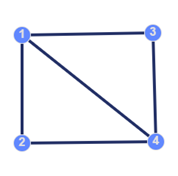
\includegraphics[width=0.17\textwidth]{imgs/Figura3}
    \caption{Exemplo de grafo simples\label{fig:imagem3}}
\end{figure}
\linebreak
- \underline{Multigrafo}, no caso de terem várias arestas a conectar os mesmos dois vértices, ou no caso de um vértice possuir um lacete, ou seja, uma “aresta” a ligar esse mesmo vértice nas duas extremidades.
\begin{figure}[h]
    \centering
    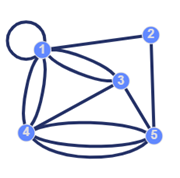
\includegraphics[width=0.17\textwidth]{imgs/Figura4}
    \caption{Exemplo de multigrafo com lacete\label{fig:imagem4}}
\end{figure}
\linebreak
\flushright{\scriptsize{(Nas companhias aéreas os passageiros detestam lacetes.\\O avião descola do aeroporto e pouco\\depois aterra no mesmo novamente!)}}

\subsection{Digrafos ou grafos orientados}
São grafos que apresentam na sua totalidade arestas orientadas, mais conhecidas como arcos.
\linebreak
\begin{figure}[h]
    \centering
    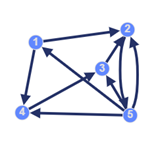
\includegraphics[width=0.2\textwidth]{imgs/Figura5}
    \caption{Exemplo de multigrafo com lacete\label{fig:imagem5}}
\end{figure}

\subsection{Grafo Parcial e Subgrafo gerado de um dado grafo}
- \underline{Grafo Parcial}: supressão de arestas, mantendo o número de vértices. Em contexto, podemos assumir 
que uma rota de voo é descontinuada por existir uma outra que implique escala ou por ser uma escala que já 
não faça sentido e exista uma outra rota direta para um dado destino.
\linebreak
\begin{figure}[h]
    \centering
    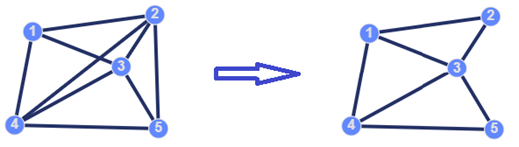
\includegraphics[width=0.2\textwidth]{imgs/Figura6}
    \caption{Exemplo de multigrafo com lacete\label{fig:imagem6}}
\end{figure}
\linebreak
- \underline{Subgrafo}: supressão de vértices e por consequência de todas as arestas com ligações a esses vértices. 
Em contexto, um destino deixa de servir os interesses da companhia, sendo canceladas como consequência 
todas as rotas para esse mesmo destino.
\linebreak
\begin{figure}[h]
    \centering
    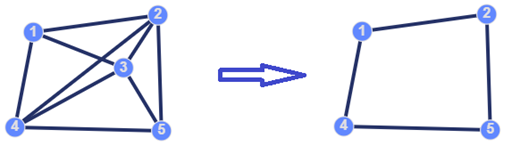
\includegraphics[width=0.2\textwidth]{imgs/Figura7}
    \caption{Exemplo de multigrafo com lacete\label{fig:imagem7}}
\end{figure}

\subsection{Grafo Subjacente e digrafo associado}
Quando queremos representar um Digrafo Associado a um dado grafo, na prática cada aresta ligada a 
dois vértices duplica, e as novas arestas passam a ter orientações opostas, aplicando-se o mesmo para os 
lacetes.
\indent Para representar um Grafo Subjacente a partir de um Digrafo, simplesmente tiramos as orientações aos 
arcos, tornando-se arestas paralelas e lacetes existentes desaparecem.
\indent Nas seguintes figuram podemos observar os conceitos de digrafo associado a um grafo e de grafo 
subjacente a um digrafo:
\linebreak
\begin{figure}[h]
    \centering
    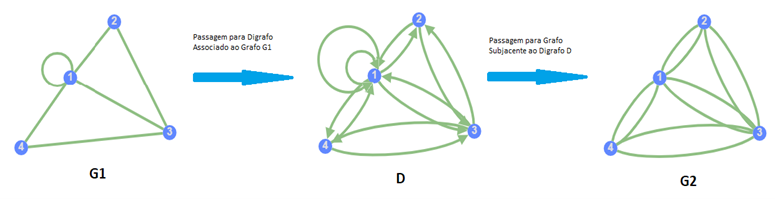
\includegraphics[width=0.2\textwidth]{imgs/Figura8}
    \caption{Exemplo de multigrafo com lacete\label{fig:imagem8}}
\end{figure}